% study2.tex -- Section V, Study 2 (writer W2, 2026-10-30). Binding contract: paper2-tnnls/SPEC.md v2.2.
% Sources: SAP-ADDENDUM-A6-LRF-2026-10-29.md A6.2-A6.6, A6.12 (branch A sentences, placement, must-not), A6.13 (disclosure, once, here)
% plus the D0094 clause (research/ledgers/decisions.jsonl); GATE-AUDIT-FAMILY-L, -LG, -BASELINES-PARITY (2026-10-30); REDTEAM-SPEC F6-F16,
% F21, F29; ABSTRACT-RULING (sentence forms).
% Rules kept here: w_j only in this section; no Study 1 symbol, role or result outside the A6.13 disclosure of V-A; features by formula
% (tables/tab_features.tex), never by any role elsewhere; no comparison of LRF with any other method; "confirmed" only for L1; no
% in-sample or design-item accuracy of the frozen object; "reliability-aware" is the method's name only. Every number has a "% run:".

\section{Study 2: Learned Reliability-Aware Fusion of Token Evidence}\label{sec:study2}
Study~2 answers Q2 (\cref{sec:intro}); the tested weighting of the evidence $\Delta_j$ is called learned reliability-aware fusion
(LRF), a name that describes its design, not a measured property.

\subsection{Provenance of the Tested Method}\label{sec:study2-provenance}
% run: git commits 941a260b (SAP A6 r1, 2026-10-29 14:40), 24d36a8a (re-frozen object, 21:00:13), 4be79be8 (fresh fold, 21:01:03);
% run: runs/P2-LRF-FROZEN-LFIX/HASHES.json:new.runs/P2-LRF-FROZEN-LFIX/model.npz (= db7fdb4e...); decision D0094 (clause on what was seen)
Study~2 was added after Study~1 had been analysed (primary result negative), when the target venue changed.
The method it tests was designed post hoc on Study~1's 500 test items.
Before the design, Study~1's primary and secondary results, its positive-control audit, its exploratory comparators, and an exploratory
learned-weighting analysis had all been seen.
In that analysis four learned-weighting families (a logistic generalised additive model, gradient-boosted trees, a multilayer perceptron,
and a grid model) were compared, and the logistic generalised additive model was selected by inner cross-validation.
Two other method designs and two other project routes were considered and not pursued.
A first freeze was found to read the true caption's length through the layout of its inputs; the caption slot was therefore fixed, and
the method was re-scored and re-frozen at that slot length, a choice declared before any re-frozen result existed.
Before the re-freeze the analysts had also seen the result table of Study~1's re-infilling family, the result of its family~B, and the
code of the decision rule of its family~H; the re-freeze protocol itself had been fixed earlier and was not changed.
The configuration was frozen (SHA-256 \texttt{db7fdb4e\ldots}, commit \texttt{24d36a8a}) before any Study~2 image was selected.
Study~2 was preregistered (a dated addendum to the analysis plan, commit \texttt{941a260b}) with a rule that no further confirmatory study would be added.
All LRF numbers on Study~1's items are post hoc and exploratory and appear only in supplement S-IV.
Study~2 tests a different method on different images and does not bear on Study~1's conclusion.

\subsection{The Frozen Weighting}\label{sec:study2-method}
Reliability-weighted fusion gives each source of evidence a weight that depends on its
reliability~\cite{chair1986optimal,kittler1998combining,zhang2023provable,han2023trusted,li2026tcpfmc}, and attention-based
multiple-instance pooling learns instance weights from instance features under a bag-level loss~\cite{ilse2018attention}.
LRF applies this construction to the per-token evidence of a unified masked diffusion model: an additive model maps features of each
image token to a non-negative weight, and the decision is the sign of the weighted evidence.

\paragraph*{Features}
Each token has 35 features in the seven groups of \cref{fig:lrf_weights}(a) (formulas in supplement S-IV).
One group holds seven token scores (five computed by the model with the caption masked, a patch-texture score, and a codebook-neighbour
distance), one holds the token's grid position, and the other five summarise the scores over a neighbourhood or the image.
% run: runs/P2-LRF-FROZEN-LFIX/spec.json:inputs_never_used (Delta, Lambda, captions, z, condition identity)
No feature uses $\Delta_j$, the caption-visible log-probabilities, the captions, the corruption labels, or the identity of the condition.
Features are standardised with the means and standard deviations of the design tokens.

\paragraph*{Weight model and decision}
For token $j$ with standardised features $x_{j1},\dots,x_{j,35}$, the weight is a logistic generalised additive model~\cite{hastie1990generalized} with a hinge basis,
\begin{equation}
w_j=\operatorname{sigm}\Big(\beta_0+\sum_{k=1}^{35}a_kx_{jk}+\sum_{k=1}^{35}\sum_{l=1}^{Q}c_{kl}\,(x_{jk}-t_{kl})_+\Big),
\label{eq:lrf-weight}
\end{equation}
where $\operatorname{sigm}$ is the logistic function and the knots $t_{kl}$ are the $l/(Q+1)$ quantiles of feature $k$ over the design tokens.
The decision and the normalised margin are
\begin{equation}
Y_{\rm LRF}=\ind\Big[\sum_{j=1}^{m}w_j\Delta_j>0\Big],\qquad M=\frac{\sum_jw_j\Delta_j}{\sum_jw_j},
\label{eq:lrf-decision}
\end{equation}
with a tie counted as wrong.
\paragraph*{Objective and tuning}
The parameters minimise, over the item-conditions of the design set,
\begin{equation}
\frac1N\sum_{i=1}^{N}\log\big(1+e^{-M_i/T}\big)+\lambda\big(\|a\|^2+\|c\|^2\big),
\label{eq:lrf-objective}
\end{equation}
a softplus loss on the margin $M_i$ of \cref{eq:lrf-decision}, which is positive when the true caption is chosen.
% run: runs/P2-LRF-FROZEN-LFIX/spec.json:T (= 0.1697); objective; hpo.method; selected_cfg.{knots,ridge,lr}; epochs (= 40); n_items (= 500)
The temperature is $T=0.170$; optimisation is AdamW without weight decay on mini-batches of 32 item-conditions.
The configuration selected by successive halving on three inner folds of the 500 design items (search in supplement S-IV; $Q=8$ knots,
$\lambda=0.0027$, learning rate 0.0169) was refitted on all 500 items for 40 epochs with a fixed seed.
% run: runs/P2-LRF-FROZEN-LFIX/spec.json:training_conditions (= clean, jpeg10, noise0.1, splice128)
The training data were the 500 design images, each scored clean, after JPEG compression at quality~10, with Gaussian noise of standard
deviation 0.1, and with a 128-pixel splice; these are also the four tested conditions.

\paragraph*{Fixed caption slot and hashes}
% run: runs/P2-LRF-FROZEN-LFIX/spec.json:caption_slot_len (= 13); rescore_checks.{invariance_max_abs_diff,positive_control_max_abs_diff,n_check}
The caption-masked scores are computed with the caption slot filled by 13 padding tokens, so they do not depend on the length of either
caption; $\Delta_j$ keeps each caption at its own length (invariance checks in supplement S-IV).
% run: runs/P2-LRF-FROZEN-LFIX/HASHES.json:new.* (model db7fdb4e..., spec 9d196d71...); pinned_vs_A6.2_table.* (all equals_table true)
The model file and every input of the scorer are pinned by SHA-256 and checked before each item (supplement S-I).
\Cref{fig:lrf_weights} draws the model and shows the learned shapes and three example weight maps.

\begin{figure*}[!t]
\centering
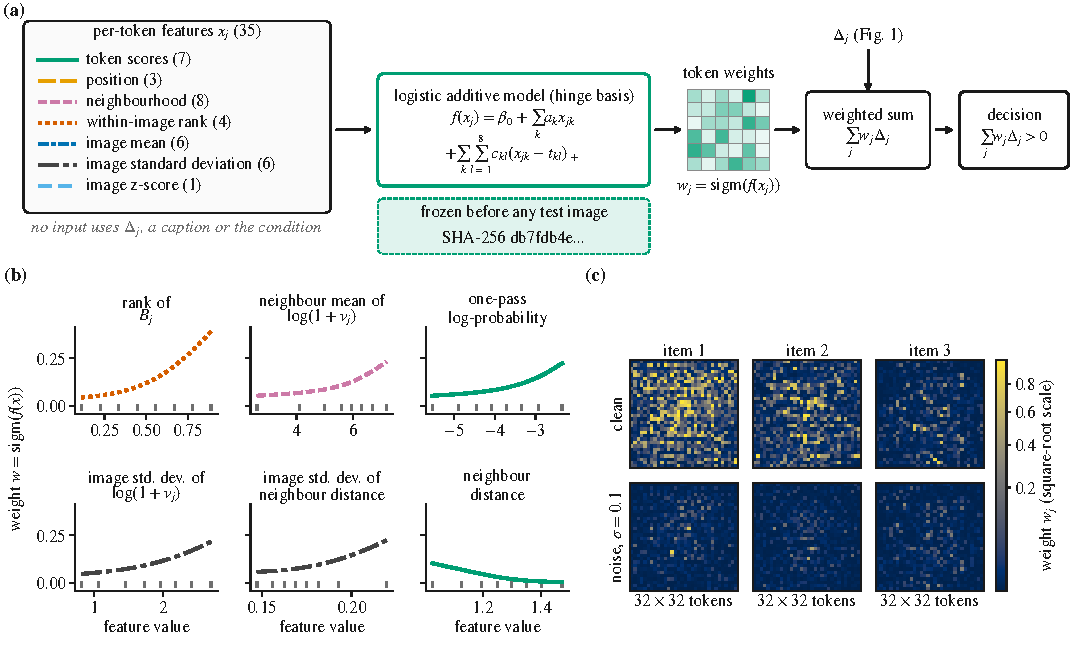
\includegraphics[width=\textwidth]{figures/fig4_study2_weights.pdf}
% run: runs/P2-LRF-FROZEN-LFIX/{model.npz,spec.json,HASHES.json} (features (35; group counts 7, 3, 8, 4, 6, 6, 1), knots, inputs_never_used, model.npz db7fdb4e...); runs/P2-LRF-L1/arrays/item000{0,1,2}.npz; values runs/P2-PAPER-FIGS/{fig4_pd_curves.json,fig4_token_weights.npz,fig4_meta.json}
\caption{Study 2: learned reliability-aware fusion (LRF) and its frozen weight model. (a) Schematic (no data; fixed weight grid). Each
image token has 35 features $x_j$ in seven groups (counts as printed; formulas in supplement S-IV); no feature uses $\Delta_j$, a caption,
or the identity of the condition. A logistic additive model with a hinge basis \eqref{eq:lrf-weight} gives the weight $w_j$, and the true
caption is chosen if $\sum_jw_j\Delta_j>0$ \eqref{eq:lrf-decision}. (b) Partial dependence of $w$ on the six of 35 features with the largest learned effect range, every other
standardised feature at its mean 0 (knots: grey ticks; line style: feature group of (a)). (c) Token-weight maps on the $32\times32$ grid
for the first three items of the fold file (chosen by position, not outcome), clean (top) and under Gaussian noise with standard
deviation 0.1 (bottom), on one square-root colour scale. Descriptive; not evidence that the weights track corruption.}
\label{fig:lrf_weights}
\end{figure*}

\begin{table*}[!t]
\centering
\caption{Study 2 Preregistered Families on the Fresh Fold: Accuracy Without and With LRF, Discordant Counts, $p$-Values, and Decisions}
\label{tab:study2}
% run: runs/P2-LRF-LG/a6_analysis.json:family_LG.cells.impulse_noise3.{p_two (= 0.058),ci95 (= [0.0, 0.1])}; family_L.L-LEN.n (= 449)
\footnotesize
\setlength{\tabcolsep}{3pt}
\resizebox{\textwidth}{!}{% tab2_study2.tex: generated by paper2-tnnls/scripts/tab2_study2.py from committed runs/ files. Do not edit by hand.
% requires booktabs; table* or adjustbox for the 9-column width
% p one-sided / p two-sided: exact McNemar p (run keys p_one, p_two); p Holm: key p_holm where the preregistration applies Holm (L3, L4 after the L1 gate; LG, m = 3), otherwise --
% L-NI: no p is printed; its preregistered test is the lower 90% bound against the margin, and superiority on clean images was not preregistered
% dagger: 90% interval (non-inferiority); every other interval 95% percentile bootstrap over items, 10000 resamples
% bold: the preregistered test of the row rejected its null at its preregistered level
\begin{tabular}{@{}lrccrrlrrrl@{}}
\toprule
Hypothesis & $n$ & Acc.\ none & Acc.\ LRF & $b$ & $c$ & Net (95\% interval) & $p$ one-sided & $p$ Holm & $p$ two-sided & Preregistered decision \\
\midrule
% run: runs/P2-LRF-L1/a6_analysis.json family_L.L1.{n,acc_a,acc_b,b,c,net,ci95,p_one,label}
% run: runs/P2-LRF-L1/a6_analysis.json branch.branch (= A)
L1: noise, $\sigma=0.1$ & 450 & 0.733 & 0.802 & 58 & 27 & \textbf{0.069} $[0.029,\,0.109]$ & 0.0005 & -- & 0.001 & \textbf{confirmed (one-sided)} \\
% run: runs/P2-LRF-L1/a6_analysis.json family_L.L3.{n,acc_a,acc_b,b,c,net,ci95,p_holm,rejected}
L3: JPEG, quality 10 & 450 & 0.849 & 0.864 & 27 & 20 & 0.016 $[-0.013,\,0.044]$ & 0.191 & 0.382 & 0.382 & not rejected \\
% run: runs/P2-LRF-L1/a6_analysis.json family_L.L4.{n,acc_a,acc_b,b,c,net,ci95,p_holm,rejected}
L4: splice, 128 px & 450 & 0.896 & 0.927 & 24 & 10 & \textbf{0.031} $[0.007,\,0.058]$ & 0.012 & 0.049 & 0.024 & \textbf{rejected (Holm)} \\
% run: runs/P2-LRF-L1/a6_analysis.json family_L.L-NI.{n,acc_a,acc_b,b,c,net,ci90,lower90,margin,non_inferior}
L-NI: clean images & 450 & 0.887 & 0.918 & 27 & 13 & 0.031 $[0.009,\,0.053]$$^{\dagger}$ & -- & -- & -- & non-inferior (lower bound 0.009 above $-0.03$) \\
% run: runs/P2-LRF-L1/a6_analysis.json family_L.L-LEN.{n,acc_a,acc_b,b,c,net,ci95,p_one,rejected} (n = 449: one item excluded)
L-LEN: noise, length-matched negatives & 449 & 0.708 & 0.784 & 67 & 33 & \textbf{0.076} $[0.033,\,0.120]$ & 0.0004 & -- & 0.0009 & \textbf{rejected (one-sided)} \\
\midrule
% run: runs/P2-LRF-LG/a6_analysis.json family_LG.cells.shot_noise3.{n,acc_a,acc_b,b,c,net,ci95,p_holm,rejected}
LG: shot noise & 300 & 0.673 & 0.767 & 43 & 15 & \textbf{0.093} $[0.047,\,0.143]$ & 0.0002 & 0.0005 & 0.0003 & \textbf{rejected (Holm, one-sided)} \\
% run: runs/P2-LRF-LG/a6_analysis.json family_LG.cells.impulse_noise3.{n,acc_a,acc_b,b,c,net,ci95,p_holm,rejected}
LG: impulse noise & 300 & 0.700 & 0.750 & 35 & 20 & \textbf{0.050} $[0.000,\,0.100]$ & 0.029 & 0.029 & 0.058 & \textbf{rejected (Holm, one-sided)} \\
% run: runs/P2-LRF-LG/a6_analysis.json family_LG.cells.speckle_noise3.{n,acc_a,acc_b,b,c,net,ci95,p_holm,rejected}
LG: speckle noise & 300 & 0.697 & 0.757 & 32 & 14 & \textbf{0.060} $[0.017,\,0.103]$ & 0.006 & 0.011 & 0.011 & \textbf{rejected (Holm, one-sided)} \\
\bottomrule
\end{tabular}
% LG impulse row: two-sided p 0.058 and 95% interval lower bound 0.0 must be stated beside it in the text (GATE-AUDIT-FAMILY-LG F2); run: runs/P2-LRF-LG/a6_analysis.json family_LG.cells.impulse_noise3.{p_two,ci95}
}

\vspace{2pt}
\parbox{\textwidth}{\scriptsize $b$: items LRF answers correctly and the unweighted rule incorrectly; $c$: the reverse; net $=(b-c)/n$.
Intervals: 95\% paired percentile bootstrap (10\,000 resamples), except $^{\dagger}$ (L-NI): 90\%, margin $-0.03$ fixed after an
exploratory clean interval had been seen; L-NI's test is the lower 90\% bound against the margin, so no $p$ is printed. $p$: exact
McNemar; $p$ Holm: L3 and L4 after L1 (two-sided), LG over its three cells (one-sided). Bold: null rejected at the preregistered level.}
\end{table*}

\begin{figure*}[!t]
\centering
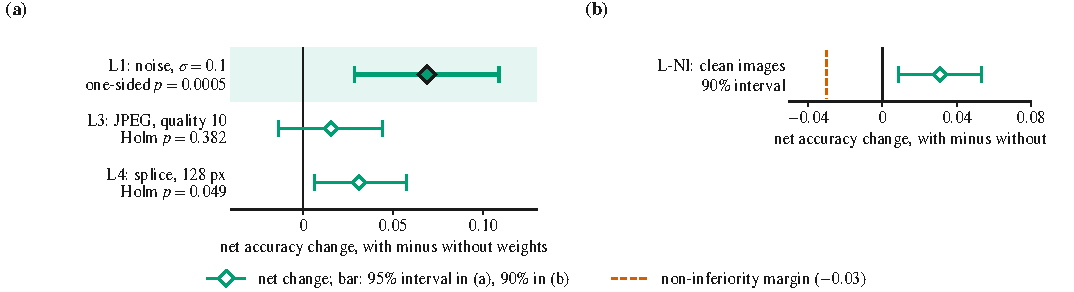
\includegraphics[width=\textwidth]{figures/fig5_study2_results.pdf}
\caption{Family L and L-NI on the fresh fold: net accuracy change of the frozen LRF, with minus without reliability weights, $n=450$.
(a) Diamond: net change; bar: 95\% paired percentile bootstrap interval. L1 (Gaussian noise, standard deviation 0.1; primary,
shaded): exact one-sided McNemar $p$; L3 (JPEG quality 10) and L4 (128-px splice): Holm-adjusted two-sided $p$. (b) L-NI (clean images;
own family): net change, 90\% interval, and the margin $-0.03$ (dashed), fixed after an exploratory clean interval had been seen.}
\label{fig:lrf_results}
\end{figure*}

\subsection{Preregistered Protocol}\label{sec:study2-protocol}
\paragraph*{Fresh fold and sample size}
% run: runs/P2-LRF-FOLD/manifest.json:meta.{n_excluded (= 2526),universe.n_eligible_images (= 2449)}; builder_report.json:n (= 533)
The fold was built after the object commit: 533 COCO val2017 images in a seeded order, drawn from the 2\,449 eligible images that remain
after the exclusions of \cref{sec:setting-data} (2\,526 image ids, some outside the captioned set) and the removal of images without
instance annotations.
% run: runs/P2-LRF-FOLD/folds_lrf.json:test[*].neg_restricted (533 of 533 true); manifest.json:length_matching.n_unrestricted (= 0)
% run: runs/P2-PAPER-TABLES/negatives_check.json:study2.{n_items (= 533), n_category_disjoint (= 533), n_fallback (= 0)}
Each image has one seeded true caption of 5 to 32 tokens, a wrong caption drawn by the preregistered derangement rule (a random caption of
another fold image sharing no annotated COCO category with it), and a second, length-matched wrong caption drawn under the same
category rule.
The fold, its eight-check leak test (with an injected leak as positive control), and the code passed automated audits run in the
authors' own pipeline (not independent reviews) before the first item.
% run: runs/P2-LRF-PLAN/n_rule.json:{n_L (= 450),rule,reason}; runs/P2-LRF-PLAN/family.json:n_rule.test_fold (= 450)
A preregistered power rule, committed before the first item, fixed the test size as a prefix of the ordered list, so it could not select
items: $n_L=450$ (its inputs are in supplement S-IV).

\paragraph*{Arms, families, and tests}
% run: design constants of research/paper2/prereg/SAP-ADDENDUM-A6-LRF-2026-10-29.md A6.4, A6.5, A6.7 (levels, margin -0.03, severity 3, n 300)
The arms are none (weight one on all 1\,024 tokens) and LRF, under clean images and the three corruptions of
\cref{sec:setting-corruptions}.
Family~L has three hypotheses, tested in a fixed sequence followed by Holm (familywise level 0.05).
The primary L1 tests LRF against none under noise by the exact one-sided McNemar test at 0.05 and is ``confirmed'' if and only if
$p\le0.05$ and $b>c$.
Only if L1 is confirmed are L3 (JPEG) and L4 (splice) tested, by exact two-sided McNemar tests with Holm over two.
A gain claim in the title, abstract, or highlights required L1 one-sided $p\le0.025$.
L-NI (one hypothesis, regardless of L1) tests non-inferiority on clean images with margin $-0.03$, read from the lower bound of the 90\%
paired bootstrap interval; the margin was fixed after an exploratory clean interval had been seen.
L-LEN (one hypothesis) repeats L1 with the length-matched wrong captions; items whose length-matched caption still differs in length are
excluded and counted.
Family~LG (Holm over three, one-sided 0.05) tests LRF against none on other noise types (shot, impulse, speckle; imagecorruptions severity
3)~\cite{michaelis2019imagecorruptions} on the first 300 fold items.
Shot and speckle noise are close relatives of Gaussian noise, impulse noise is the structurally different cell, and severity 3 is not
matched to $\sigma=0.1$.
According to the operations log, no output was read before its run was complete.

\subsection{Results}\label{sec:study2-results}
% run: runs/P2-LRF-L1/a6_analysis.json:multiplicity_note (no adjustment across families); 17 families: SAP-ADDENDUM-A6 A6.7 (D0100)
\Cref{tab:study2} gives every preregistered test and \cref{fig:lrf_results} the family-L intervals; each family is at its own level, with
no adjustment across families (\cref{sec:setting-tests}).
% run: runs/P2-LRF-L1/a6_analysis.json:family_L.*.{n_d,ci90,cp95_b_over_nd,p_mid_one,p_mid_two}; runs/P2-LRF-LG/a6_analysis.json:family_LG.cells.* (table tables/supp_tests_full_study2.tex)
The remaining quantities that the plan reports with every test ($n_d$, 90\% intervals, the Clopper--Pearson interval of $b/n_d$ and
the mid-$p$ values) are in supplement S-IV.
% run: runs/P2-LRF-L1/a6_analysis.json:family_L.L1.{acc_b (= 0.7333),acc_a (= 0.8022),net,ci95,p_one,label (= confirmed)}; branch.branch (= A)
On a fresh preregistered fold, the frozen LRF raised image-direction verification accuracy under Gaussian noise ($\sigma=0.1$) from 0.733
without reliability weighting to 0.802 (net 0.069, 95\% interval 0.029 to 0.109; exact one-sided McNemar $p=0.0005$; preregistered
one-sided $\alpha=0.05$), including with length-matched negatives
% run: runs/P2-LRF-L1/a6_analysis.json:family_L.L-LEN.{n,acc_b,acc_a,net,ci95,p_one,n_excluded_length_mismatch,label}
(0.708 to 0.784, net 0.076, 0.033 to 0.120; one-sided $p=0.0004$; $n=449$, one item excluded for a length mismatch).
L1 is therefore confirmed.
This result holds in one pretrained unified masked diffusion model (UniDisc, 1.4B parameters), on 450 COCO val2017 images not used to design or fit
the method, with Gaussian noise at one severity.
% run: runs/P2-LRF-L1/a6_analysis.json:family_L.L-NI.{acc_b (= 0.8867),acc_a (= 0.9178),net,ci90,lower90,margin,non_inferior,margin_note}
On clean images LRF lost no more than three percentage points (0.03 in accuracy; 90\% interval of the net change 0.009 to 0.053); the margin was fixed after an
exploratory clean interval had been seen.
The clean-image estimate, descriptive, was positive (0.887 without weighting, 0.918 with; net 0.031); superiority on clean images was not a
preregistered hypothesis.
Supplement S-IV plots the discordant items of L1 and of the clean cell by margin (descriptive).

% run: runs/P2-LRF-L1/a6_analysis.json:family_L.L3.{net,ci95,p_holm}
Under JPEG quality~10 no difference was detected (net 0.016, 95\% interval $-0.013$ to $0.044$; Holm-adjusted $p=0.382$).
% run: runs/P2-LRF-L1/a6_analysis.json:family_L.L4.{acc_b,acc_a,net,ci95,p_two,p_holm (= 0.0486)}
Under the 128-pixel splice LRF raised accuracy from 0.896 to 0.927 (net 0.031, 0.007 to 0.058); the Holm-adjusted $p$ is 0.049,
0.001 below the 0.05 level (unadjusted two-sided $p=0.024$).
% run: runs/P2-LRF-L1/a6_analysis.json:family_L.*.harm (all false); runs/P2-LRF-LG/a6_analysis.json:family_LG.cells.*.harm (all false)
No tested condition showed a reduction: the lowest 95\% bound was $-0.013$, under JPEG.

% run: runs/P2-LRF-LG/a6_analysis.json:family_LG.cells.shot_noise3.{acc_b,acc_a,net,ci95,p_one,p_holm,p_two}
% run: runs/P2-LRF-LG/a6_analysis.json:family_LG.cells.speckle_noise3.{acc_b,acc_a,net,ci95,p_one,p_holm,p_two}
% run: runs/P2-LRF-LG/a6_analysis.json:family_LG.cells.impulse_noise3.{acc_b,acc_a,net,ci95,p_one,p_holm,p_two}
% D0099 (factual sentence; not a held-out or transfer claim): runs/P2-LRF-FROZEN-LFIX/spec.json:training_conditions (= clean, jpeg10, noise0.1, splice128)
None of the three other noise types (shot, impulse, speckle; imagecorruptions severity 3) was a training condition of the frozen
weighting (training conditions: clean, JPEG quality~10, Gaussian noise 0.1, 128-pixel splice).
Shot and speckle noise are close relatives of Gaussian noise, impulse noise is the structurally different cell, and severity 3 is not
matched to $\sigma=0.1$; no claim is made about corruption types not tested.
On these types ($n=300$ each), each LG hypothesis was rejected with $b>c$.
Under shot noise accuracy rose from 0.673 to 0.767 (net 0.093, 0.047 to 0.143; one-sided $p=0.0002$, Holm-adjusted $p=0.0005$, two-sided
$p=0.0003$), and under speckle noise from 0.697 to 0.757 (net 0.060, 0.017 to 0.103; one-sided $p=0.006$, Holm-adjusted $p=0.011$, two-sided $p=0.011$).
Under impulse noise it rose from 0.700 to 0.750 (net 0.050), and the 95\% interval has lower bound 0.0 (0.000 to 0.100).
The one-sided and Holm-adjusted $p$-values are both 0.029, and the two-sided $p$ is 0.058, so this cell would not pass a two-sided 0.05 test, and no
two-sided claim is made for it.
The three cells are reported separately and are not pooled.

\subsection{Reference Encoders}\label{sec:study2-reference}
% run: runs/P2-LRF-BASELINES/baselines.json:table.{clip,siglip}.*.acc (range 0.996 to 1.000); models.* (pinned revisions)
For reference, CLIP ViT-L/14~\cite{radford2021clip} and SigLIP so400m~\cite{zhai2023sigmoid}, different models trained on different data, reached accuracies of 0.996 to 1.000 on the
same items in every condition (\cref{tab:baselines}), with the same decision rule on images regenerated with the runner's corruption
functions and seeds (supplement S-VI).
% run: runs/P2-LRF-BASELINES-PARITY-L1/baselines.json:pixel_parity.{min (= 0.989),threshold}; runs/P2-LRF-BASELINES-PARITY-LG/baselines.json:pixel_parity.{min (= 0.986),threshold}
Pixel parity was shown: the UniDisc tokeniser's re-encoding of the regenerated images agreed with the stored codes on at least 98.6\% of
tokens (five items per condition set; threshold 98\%).
Nearly every cell is at or next to its ceiling, so no reading beyond the stated accuracies is drawn, and no test is made.

\begin{table}[!t]
\centering
\caption{Reference Accuracy of CLIP ViT-L/14 and SigLIP so400m per Condition}
\label{tab:baselines}
\footnotesize
\setlength{\tabcolsep}{2pt}
\resizebox{\columnwidth}{!}{% tab3_baselines.tex: generated by paper2-tnnls/scripts/tab3_baselines.py from committed runs/ files. Do not edit by hand.
% drop: clean minus corrupted accuracy of the same model on the same items (paired percentile bootstrap, 95% interval, from baselines.json)
% no test, no ranking, no LRF number in this table (A6.6); nothing bold
% stale field: runs/P2-LRF-BASELINES/baselines.json pixel_parity says 'not run' because the main run was made without --parity; the parity runs P2-LRF-BASELINES-PARITY-L1 and -LG supersede it
% models: openai/clip-vit-large-patch14 rev 32bd6428..., google/siglip-so400m-patch14-384 rev 9fdffc58... (runs/P2-LRF-BASELINES/baselines.json models.*)
\begin{tabular}{@{}lrcccc@{}}
\toprule
Condition & $n$ & CLIP acc. & CLIP drop (95\% interval) & SigLIP acc. & SigLIP drop (95\% interval) \\
\midrule
% run: runs/P2-LRF-BASELINES/baselines.json table.clip.clean.{n,acc,drop,drop_ci95}; table.siglip.clean.{acc,drop,drop_ci95}
Clean images & 450 & 0.998 & -- & 0.998 & -- \\
% run: runs/P2-LRF-BASELINES/baselines.json table.clip.noise0.1.{n,acc,drop,drop_ci95}; table.siglip.noise0.1.{acc,drop,drop_ci95}
Gaussian noise, $\sigma=0.1$ & 450 & 1.000 & $-0.002$ $[-0.007,\,0.000]$ & 0.998 & 0.000 $[0.000,\,0.000]$ \\
% run: runs/P2-LRF-BASELINES/baselines.json table.clip.jpeg10.{n,acc,drop,drop_ci95}; table.siglip.jpeg10.{acc,drop,drop_ci95}
JPEG, quality 10 & 450 & 0.998 & 0.000 $[0.000,\,0.000]$ & 1.000 & $-0.002$ $[-0.007,\,0.000]$ \\
% run: runs/P2-LRF-BASELINES/baselines.json table.clip.splice128.{n,acc,drop,drop_ci95}; table.siglip.splice128.{acc,drop,drop_ci95}
Splice, 128 px & 450 & 0.996 & 0.002 $[0.000,\,0.007]$ & 1.000 & $-0.002$ $[-0.007,\,0.000]$ \\
\midrule
% run: runs/P2-PAPER-TABLES/baselines_clean300.json models.{clip,siglip}.{n,acc}
Clean images, same 300 items & 300 & 0.997 & -- & 0.997 & -- \\
% run: runs/P2-LRF-BASELINES/baselines.json table.clip.shot_noise3.{n,acc,drop,drop_ci95}; table.siglip.shot_noise3.{acc,drop,drop_ci95}
Shot noise, severity 3 & 300 & 1.000 & $-0.003$ $[-0.010,\,0.000]$ & 0.997 & 0.000 $[0.000,\,0.000]$ \\
% run: runs/P2-LRF-BASELINES/baselines.json table.clip.impulse_noise3.{n,acc,drop,drop_ci95}; table.siglip.impulse_noise3.{acc,drop,drop_ci95}
Impulse noise, severity 3 & 300 & 0.997 & 0.000 $[0.000,\,0.000]$ & 0.997 & 0.000 $[0.000,\,0.000]$ \\
% run: runs/P2-LRF-BASELINES/baselines.json table.clip.speckle_noise3.{n,acc,drop,drop_ci95}; table.siglip.speckle_noise3.{acc,drop,drop_ci95}
Speckle noise, severity 3 & 300 & 1.000 & $-0.003$ $[-0.010,\,0.000]$ & 0.997 & 0.000 $[0.000,\,0.000]$ \\
\midrule
% run: runs/P2-LRF-BASELINES/baselines.json holds no timing; runs/P2-LRF-BASELINES.stdout.txt and .stderr.txt hold none
Cost per item & -- & \multicolumn{4}{l}{not measured (no timing in any committed baseline run)} \\
\midrule
% run: runs/P2-LRF-BASELINES-PARITY-L1/baselines.json pixel_parity.{min,threshold,ok}, n_items
\multicolumn{6}{l}{Pixel parity, 5 items, the four conditions of the top block: minimum token agreement 0.989 (threshold 0.98)} \\
% run: runs/P2-LRF-BASELINES-PARITY-LG/baselines.json pixel_parity.{min,threshold,ok}, n_items
\multicolumn{6}{l}{Pixel parity, 5 items, clean and three severity-3 conditions: minimum token agreement 0.986 (threshold 0.98)} \\
\bottomrule
\end{tabular}
}

\vspace{2pt}
\parbox{\columnwidth}{\scriptsize For reference only: different models trained on different data; no test and no comparison are made.
Same first 450 fold items (300 for the severity-3 cells) and regenerated pixels; revisions and scores in supplement S-VI. Drop: clean minus corrupted accuracy of the same model on the same items, paired percentile bootstrap 95\% interval. The row
``Clean images, same 300 items'' was computed at writing from the stored predictions (descriptive). Cost per item was not measured.
Pixel parity: \nolinkurl{runs/P2-LRF-BASELINES-PARITY-L1} and \nolinkurl{-LG}; these supersede the field
\nolinkurl{pixel_parity: not run} of the main run's file, which records only that the main run was made without the parity option.}
\end{table}

\subsection{Cost of Study 2}\label{sec:study2-cost}
% run: runs/P2-LRF-L1/items.jsonl:n_rows, seconds, peak_gb (67 rows, median 8.0 s, max 8.2 GB); runs/P2-LRF-LG/items.jsonl (42 rows, 5.0 s)
The fresh-fold pass, which computes the unweighted rule for four conditions and stores the inputs of LRF, used 67 network rows and a median of 8.0~s per item on one 12~GB laptop GPU, with a peak memory of 8.2~GB; the stage of the other noise
types used 42 rows and 5.0~s per item (supplement S-IV).
LRF adds no network row; its weights and decision are computed from the stored arrays on the CPU and were not timed.

\subsection{Exploratory Ablation}\label{sec:study2-ablation}
\begin{figure}[!t]
\centering
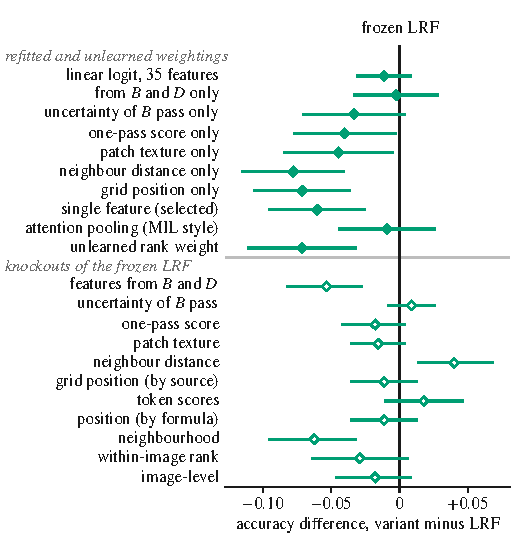
\includegraphics[width=\columnwidth]{figures/fig_ablation.pdf}
% run: runs/P2-LRF-ABL-SCORE/ablation_analysis.json:rows[*].cells.L1_noise0.1.vs_LRF.{d,ci95}; n_per_cell; ko_all_control; meta.{label,sign,interval}; values runs/P2-PAPER-FIGS/fig_ablation.json
\caption{Study 2, exploratory ablation (added after the primary, family~H, and Study~2 results; intervals only, no test): paired accuracy
difference, variant minus the frozen LRF, on the L1 noise cell ($n=450$), with the 95\% paired percentile-bootstrap interval
(10\,000 resamples). A positive value favours the variant. Upper block: weightings refitted with LRF's
protocol on the 500 design items only, and one unlearned rank weight. Lower block: knockouts, the frozen LRF with one feature group set to
its design-item mean (see the text for how a knockout interval is read). Intervals are
marginal, dependent, and unadjusted (supplement S-VII, with the other cells).}
\label{fig:ablation}
\end{figure}
% run: runs/P2-LRF-ABL-SCORE/ablation_analysis.json (commits facab605, 4e785aa9; plan research/paper2/tnnls/ABLATION-PLAN-2026-10-30.md section 8)
Exploratory; added after the primary, family~H, and Study~2 results; no ablation was preregistered, and every variant is in supplement S-VII.
Single-source refits and other weightings were fitted with LRF's protocol on the 500 design items only; knockouts set one feature group of
the frozen LRF to its design-item mean (differences are variant minus LRF; positive favours the variant).
% run: runs/P2-LRF-ABL-SCORE/ablation_analysis.json:rows[*].cells.L1_noise0.1.vs_LRF.ci95 (classification: A-LIN, A-S-BD, A-S-s3, A-MIL contain 0; A-S-tbv, A-S-ltex, A-S-nbr, A-S-pos, A-SF, A-UNL, KO-S-BD, KO-F-neighbourhood below 0; KO-S-nbr above 0; other KO rows contain 0)
\Cref{fig:ablation} shows every variant on the noise cell.
The following intervals contained zero: those of a linear logit on the same 35 features, of the features computed from $B$ and $D$ alone,
of the features from the uncertainty of the $B$ pass alone, and of attention-weighted pooling in the style of gated-attention
multiple-instance learning (MIL)~\cite{ilse2018attention}.
They lay below zero for the other single-source weightings, the unlearned rank weight, and a single-feature weight (the distance from the
grid centre, chosen from 35 candidate features by the inner-fold objective on the design items, a selection budget 35 times that of the
frozen LRF; the selection used no fresh item).
Among knockouts, the intervals for the features from $B$ and $D$ and for the neighbourhood features lay below zero and the interval for the
codebook-neighbour-distance features above it; every other group's interval contained zero.
Setting a group to its mean gives inputs that the model did not see together in fitting; an interval away from zero shows that the frozen
model's decisions depend on those inputs, not that the group alone detects anything.
% run: runs/P2-LRF-ABL-SCORE/ablation_analysis.json:seed_spread.{max_range_over_variants_and_cells (= 0.030),seed0_is_prefixed (= true)}; K (= 336)
Across the three refit seeds, the range of fresh-fold accuracy was at most 0.030 in every variant and cell; seed 0 was fixed before any
fresh item and is not the best of three.
The 336 intervals are dependent and unadjusted, and the other cells are in supplement S-VII.
